\part{Annex}

\section{Bibliographic searches}\label{Prognosis Alzheimer cerca}

We carried out a total of 5 structured search reviews. 

\textbf{Search 1} wanted to identify \textbf{any} relevant biomarkers and/or predictive/prognostic models of AD research in the MCI population via assessing review articles.

\textbf{Search 2} was exactly the same as search 1, but only screened last two years (2017 and 2018) and there was not filter by study type (i.e. review). With it we wanted to identify primary studies not covered in serach 1.

\textbf{Searches 3, 4 and 5} were designed consecutively, with same aim in mind than the previous searches. This time, however, the focus was only in fMRI as main biomarker and/or predictor, and only 2017 and 2018 as review periods.

\subsection{Search 1} \label{search1_AD_reviews}


\textit{\textbf{Search 1 (Pubmed):} (Alzheimer's[tiab] OR Alzheimer Disease[Mesh]) AND (MCI[tiab] OR "Mild cognitive impairment"[tiab] OR "Cognitive Dysfunction"[Mesh]) AND (prognosis[tiab] or prediction[tiab])}

This bibliographic search was carried out on 03/04/2018 using this descriptors: After filtering by ``Review'' we got 77 review articles. From those, we filtered again to retain only the reviews published in the last five years: we got 28 review articles. From these, since we considered the newest reviews were comprehensive enough, we only looked into review articles published within the last two natural years (2018 and 2017). Then, three reviews were excluded, since they did not answer our research questions (i.e. one assessed epilepsy in AD\footnote{https://www.ncbi.nlm.nih.gov/pubmed/28501143}, another one assessed post-stroke dementia\footnote{https://www.ncbi.nlm.nih.gov/pubmed/28095900} and the remaining assessed gait\footnote{https://www.ncbi.nlm.nih.gov/pubmed/28222369}). In total, 7 review articles were eligible to read (see \ref{whatever}\cite{Liu201856,Henriques2018,Martinez2017,Sarica2017,Dallora2017,Rathore2017530,Herukka2017285}).
\FloatBarrier

\begin{table}[h]
	\centering
	\begin{threeparttable}
		\caption{Included reviews of Search 1}
		\label{whatever}	
		\begin{tabular}{lll}
			\toprule
			\textbf{Included review\tnote{a}} & \textbf{Screening time\tnote{b}} & \textbf{Source\tnote{c}}\\
			\midrule
			Liu et al.\cite{Liu201856} & Last 10 years & Pubmed \\
			Henriques et al.(2018)\cite{Henriques2018} & No search period specified & not reported \\
			Martinez et al. (2017)\cite{Martinez2017} & Up until May 2017 & \tnote{g}\\
			Sarica et al. (2017)\cite{Sarica2017} & Last 10 years &  \tnote{d}\\
			Dallora et al.(2017)\cite{Dallora2017} & Until 23 Oct 2015\tnote{f} & \tnote{e}\\
			Rathore et al. (2017)\cite{Rathore2017530} & Jan 1985 to June 2016 & \tnote{h}\\
			Herukka et al. (2017)\cite{Herukka2017285}& No search period specified & MEDLINE \\
			\bottomrule
		\end{tabular}
		\scriptsize\begin{tablenotes} %canvia el tamany aqui
			\item[a]{identifier}
			\item[b]{The period of time the reviewers cover.}
			\item[c]{The source the reviewers took the articles from.}
			\item[d]{Pubmed, scopus, WoS and Google Scholar.}
			\item[e]{Pubmed, WoS, Scopus.}
			\item[f]{Starting period not specified. We assume no time restrictions were applied.}
			\item[g]{Several resources. among which MEDLINE, Embase, PsycINFO, ALOIS and WHO ICTRP databases were covered.}
			\item[h]{Google scholar and pubmed.}

		\end{tablenotes}
	\end{threeparttable}
	
	
	
	
	
\end{table}


%CAL CANVIAR ELS LOREM IPSUMS!!
You can see in table \ref{whatever} included reviews from search 1, their spanning literature-review search periods and their sources of information. Beyond these covered references, we added in our theoretical framework other reviews and primary articles as well. Those come from backward snowballing (which means that reference list of any of those studies was used to identify new papers to include) or by non structured means of search. For example there is an excellent review, covering since 1990 up to 2015, from Arbabshirani et al.                                           \cite{Arbabshirani2017137}, but was not identified via search 1. We found independently via a SCOPUS review, which has 100\% MEDLINE, EMBASE and COMPENDEX coverage; and the second, by downloading a volume of the Neuroimage magazine my tutor Andrea Insabatto recommended me.

\subsection{search 2}
	
This search has same syntax as search 1, but unlike search 1 we did not exclude primary studies as no filter by review was applied. We do not report which studies from this search have been added in our study:
	
		\noindent \textit{\textbf{Search 2 (Pubmed):} (Alzheimer's[tiab] OR Alzheimer Disease[Mesh]) AND (MCI[tiab] OR "Mild cognitive impairment"[tiab] OR "Cognitive Dysfunction"[Mesh]) AND (prognosis[tiab] or prediction[tiab])}

\subsection{searches 3 - 5}
	We carried out two more searches in order to detect primary studies published in the last two years (2017 and 2018). This was made since, for obvious publishing timings, none of the reviews obtained in search 1 were expected to cover the gap of primary studies published in the last two years. We could be losing articles that assess predictive models using fMRI for that reason. Which is what we really need to know.
	
	Hence, searches 3 and 4 will now have less sensitivity: because we are now just reviewing studies that use fMRI with prognostic purposes:
	
		\noindent \textit{\textbf{Search 3 (Scopus):} TITLE-ABS-KEY ( mci  AND  prognosis  AND  fmri )}\footnote{No complex descriptor usage was intended since Scopus releases a lot of noise.}
		
		\noindent \textit{\textbf{Search 4 (Pubmed):} (Alzheimer's[tiab] OR Alzheimer Disease[Mesh]) AND (MCI[tiab] OR "Mild cognitive impairment"[tiab] OR "Cognitive Dysfunction"[Mesh]) AND (prognosis[tiab] or prediction[tiab]) AND  (fMRI[tiab] OR rsfMRI[tiab])}
		
	The Scopus search (Search 3) returned six results. The Pubmed search (Search 4) only returned one result. We included in our theoretical framework four of them, and they are depicted in table \ref{whatever3}. Only one answers the exact same question as ours.
		
		\begin{table}[h]
			\centering
			\begin{threeparttable}
				\caption{Included studies in literature review 3 and 4}
				\label{whatever3}	
				\begin{tabular}{llll}
					\toprule
					\textbf{Included study\tnote{a}} & \textbf{Source\tnote{b}} & \textbf{predictor\tnote{c}} & \textbf{outcome\tnote{d}} \\
					\midrule
					Hojjati (2017)\tnote{f}\cite{Hojjati201769} & Scopus & fMRI & AD onset \\
					Tian dai (2017)\cite{Dai2017772} & Pubmed & fMRI + other & future fcon\\
					Yu et al (2016)\cite{Yu2016} & Scopus & fMRI + other & T2DM\tnote{e} \\
					Petrella et al (2017)\cite{Petrella2007} & Scopus & - & - \\
					\bottomrule
					
								
				\end{tabular}
				\scriptsize\begin{tablenotes} %canvia el tamany aqui
					\item[a]{identifier}
					\item[b]{The source we retrieved the article from}
					\item[c]{The variable used to predict}
					\item[d]{The variable its change is being predicted}
					\item[e]{Type 2 diabetes mellitus}
					\item[f]{This study is the only study we have found that answers the exact same question we have.}					
				\end{tablenotes}
			\end{threeparttable}
		\end{table}
	
	
	Finally, since the last two searches did almost not return results, we propose increasing the sensitivity of search 4 by lowering its precision: we simply remove the fMRI descriptors, and we add the Mesh descriptor``Magnetic Resonance Imaging''[Mesh]. With this we get to include in our results all neuroimaging data labeled as a Mesh descriptor, which may include fMRI (There is no specific fMRI mesh term).
	
	\noindent \textit{\textbf{Search 5 (Pubmed):} (Alzheimer's[tiab] OR Alzheimer Disease[Mesh]) AND (MCI[tiab] OR "Mild cognitive impairment"[tiab] OR "Cognitive Dysfunction"[Mesh]) AND (prognosis[tiab] or prediction[tiab]) AND "Magnetic Resonance Imaging"[Mesh]}
	
	
	Search 5 obtained 24 results. Of which we did not select anyone, since neither of them included fMRI. Thus, we can understand search 4 already had a high sensitivity when detecting studies with fMRI that assessed the topic of MCI to AD conversion.



\section{AAL: Labels} \label{AAL_annex}

Precentral-L, Frontal-Sup-L, Frontal-Sup-Orb-L, Frontal-Mid-L, Frontal-Mid-Orb-L, Frontal-Inf-Oper-L, Frontal-Inf-Tri-L, Frontal-Inf-Orb-L, Rolandic-Oper-L, Supp-Motor-Area-L, Olfactory-L, Frontal-Sup-Medial-L, Frontal-Med-Orb-L, Rectus-L, Insula-L, Cingulum-Ant-L, Cingulum-Mid-L, Cingulum-Post-L, Hippocampus-L, ParaHippocampal-L, Amygdala-L, Calcarine-L, Cuneus-L, Lingual-L, Occipital-Sup-L, Occipital-Mid-L, Occipital-Inf-L, Fusiform-L, Postcentral-L, Parietal-Sup-L, Parietal-Inf-L, SupraMarginal-L, Angular-L, Precuneus-L, Paracentral-Lobule-L, Caudate-L, Putamen-L, Pallidum-L, Thalamus-L, Heschl-L, Temporal-Sup-L, Temporal-Pole-Sup-L, Temporal-Mid-L, Temporal-Pole-Mid-L, Temporal-Inf-L, Precentral-R, Frontal-Sup-R, Frontal-Sup-Orb-R, Frontal-Mid-R, Frontal-Mid-Orb-R, Frontal-Inf-Oper-R, Frontal-Inf-Tri-R, Frontal-Inf-Orb-R, Rolandic-Oper-R, Supp-Motor-Area-R, Olfactory-R, Frontal-Sup-Medial-R, Frontal-Med-Orb-R, Rectus-R, Insula-R, Cingulum-Ant-R, Cingulum-Mid-R, Cingulum-Post-R, Hippocampus-R, ParaHippocampal-R, Amygdala-R, Calcarine-R, Cuneus-R, Lingual-R, Occipital-Sup-R, Occipital-Mid-R, Occipital-Inf-R, Fusiform-R, Postcentral-R, Parietal-Sup-R, Parietal-Inf-R, SupraMarginal-R, Angular-R, Precuneus-R, Paracentral-Lobule-R, Caudate-R, Putamen-R, Pallidum-R, Thalamus-R, Heschl-R, Temporal-Sup-R, Temporal-Pole-Sup-R, Temporal-Mid-R, Temporal-Pole-Mid-R, Temporal-Inf-R.








\section{Data recollecting}
	\subsection{Obtaining ADNI data} \label{subsec_appendix_obteniribaixarInfoADNI}

	In order to gather information about the baseline diagnosis, diagnosis disease changes, examdates where those diagnosis took place, questionnaire scores and fluid biomarkers we downloaded a file that contains subject data for commonly used variables in the ADNI, called \textit{ADNIMERGE package for SPSS}. We downloaded it on the 19/03/2018, following the instructions provided here: \cite{adni_data_training_part2} (p. 31, p. 40 - 44) \footnote{ADNIMERGE files are updated daily}. Within it, \textit{adnimerge.csv} file was used to obtain participants' phenotipic and diagnostic information, whereas lines 5 - 117 of ADNIMERGE.sps (SPSS syntax file) contained variable names to be used as column headers of the aforementioned \textit{adnimerge.csv} file. Hence, those lines were parsed using a custom python script to create a proper header for the \textit{adnimerge.csv}. \textit{adnimerge.csv} was then imported to \textit{adnimerge.sav} (SPSS statistics data document), to pandas dataframe object and to python dictionaries for further analysis and datalinkage with \textit{fMRI.csv} using Python scientific libraries.
	
	In order to get information for the fMRI scans of participants, we had to download all fMRI data. Simply, there was not a good subsampling procedure to download just specific neuroimage files for selective subjects. Thus, we were forced to download all fMRI scans acquired until 13/02/2018. This was achieved using the Image Data Archive website\footnote{\href{https://ida.loni.usc.edu/login.jsp}{https://ida.loni.usc.edu/login.jsp}}.
	
	According to the ADNI website, neuroimaging data is to be obtained following the instructions provided within ``Standardized Image Collections'' section in this page\footnote{\href{http://adni.loni.usc.edu/methods/mri-analysis/adni-standardized-data/}{http://adni.loni.usc.edu/methods/mri-analysis/adni-standardized-data/}}. However, steps 3 - 5 stated in this reference were not taken into account since they only include data from the first stage of the study (ADNI 1) -this is especially important since ADNI 1, did not yet include fMRI analysis-. We instead used the ``Advanced Search'' tab for that purpose.
	
	Within the previously mentioned ``Advanced Search'' tab we carried out an image search filtering by ``ADNI'' as study data and ``fMRI'' as imaging modality. We then identified a total of 7959 fMRI sessions. All 7959 fMRI sessions were saved as an  \textit{image collection}, and later on downloaded selecting .nii files as neuroimaging format by using the ``advanced download'' option and splitting the file in 10 .rar documents of $ \approx 8 GB$ each. Inside this image collection, an accompanying .csv file with the name of the previously created \textit{image collection} (which in the text we refer to as fMRI.csv) could be downloaded by clicking the csv button. This file has been used as stated in methods section.




\clearpage
\section{Tables} 



	\subsection{Participating centers in the baseline diagnostic of our 332 eligible participants} \label{taula_centres_metode}
	
	
	\begin{figure}[h]
		\centering
		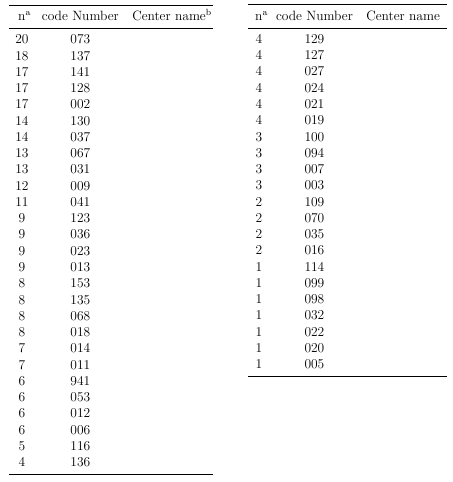
\includegraphics[width=0.80\textwidth]{tauladelscollons.png}
		\caption{\textbf{Centers at which eligible subjects were assessed at the baseline.} $| ^{a}.$ Number of subjects per center. $| ^{b}.$ We have been unable to find where the correspondence between center codes and center names is. However, the total number of centers can be found on the ADNI website.}
		\label{fig:tauladelscollons}
	\end{figure}
	\clearpage
	
	\subsection{The seven more frequent fMRI submodalities in our 332 eligible participants} \label{taula_submodalitats_fmri} 


		\begin{figure}[h]
			\centering
			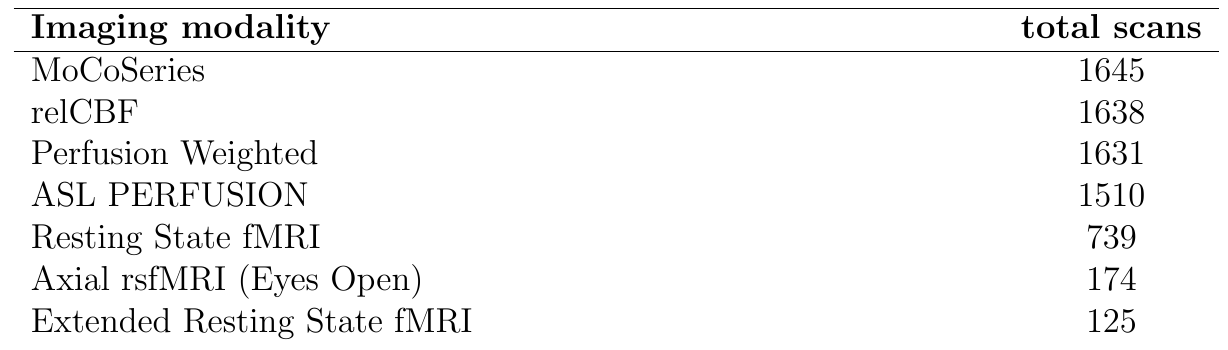
\includegraphics[width=1\textwidth]{fig_submodalitats_fmri_mesfrequents.png}
			\caption{\textbf{Value counts per submodality}, a measure of scan availability by fMRI subtype}
			\label{fig:submodalitats_fmri_mesfrequents}
		\end{figure}


	\subsection{Number of participants by site and group (results section)}\label{centres_resultats_74pacients}
		\FloatBarrier
		\begin{table}[h]
		\centering
		\begin{threeparttable}
			\caption{Number of participants and column percentages by site and group -final 74 patients sample-}
			\label{table:centres_en_mostrafinal_74 pacients}
			\begin{tabular}{ll|lll|llr}
				\toprule
				code n&site &MCI-c&MCI-nc&total&\% MCI-c&\% MCI-nc & $\sum$\%\\
				\midrule
				001&1&5&8&13&21,74&15,69&17,57\\
				130&53&4&7&11&17,39&13,73&14,86\\
				006&22&2&8&10&8,7&15,69&13,51\\
				018&13&1&6&7&4,35&11,76&9,46\\
				053&31&1&5&6&4,35&9,8&8,11\\
				013&10&2&4&6&8,7&7,84&8,11\\
				012&9&2&4&6&8,7&7,84&8,11\\
				006&4&3&3&6&13,04&5,88&8,11\\
				136&58&1&1&2&4,35&1,96&2,7\\
				129&52&0&2&2&0&3,92&2,7\\
				100&43&0&2&2&0&3,92&2,7\\
				019&14&1&1&2&4,35&1,96&2,7\\
				041&28&1&0&1&4,35&0&1,35\\
				\bottomrule
				&total&23&51&74&100&100&100\\
				\bottomrule
			\end{tabular}
			
			%\begin{tablenotes}
			%	\item[a]{asd}
			%	\item[b]{asd}
			%\end{tablenotes}
		\end{threeparttable}
	\end{table}
	
	
	
	

	\FloatBarrier
	
	
	
	\subsection{Homocedasticity and normality assumptions to support the use of statistical tests in demographics table and in FCon distribution comparisons.} \label{taula_levene_shapiro_demografics} 
	
		$H_{0}$ for \textit{shapiro wilk}: The null hypothesis, for this test, means that 
		the population of the corresponding subgroup (either MCIc or MCInc),
		for the given variable, is normally distributed. If + appears means that 
		we have to reject the Ho and thus the variable does not ajust a normal 
		distribution for that group.
		
		$H_{0}$ for \textit{levene test}: There is homogeneity of variances (both groups have
		same variance), for a given variable. If ``+'' symbol appears in figure \ref{fig:fig_shapiro_levene_taulaDEMOGRAFICS} below, it means that 
		we reject the Ho and therefore both groups are assumed not to 
		have the same variance.
		
		Thus, any variable (line) with any significant test result needs 
		the nonparametric option (Mann Whitney) [mw] instead of the parametric
		one (independent samples t-test) [t]:
		\FloatBarrier	
		\begin{figure}[h]
			\centering
			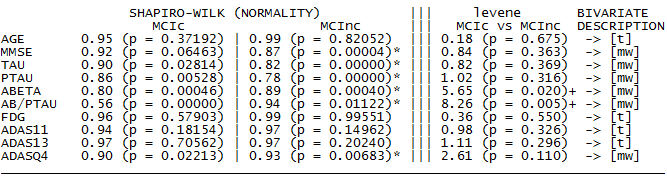
\includegraphics[width=1\textwidth]{fig_shapiro_levene_taulaDEMOGRAFICS.png}
			\caption{Assessment of the assumptions of all bivariate comparisons made in table \ref{table:demografics_biomarc_clinic_participants}.}
			\label{fig:fig_shapiro_levene_taulaDEMOGRAFICS}
		\end{figure}
		\FloatBarrier	

		Similarly, when comparing FC distributions between MCI-c and MCI-nc individuals (on the whole sample and by center), we have used the same tests to check the homocedasticity and normality assumptions before deciding which test to use. These were the results:
	
		\FloatBarrier
		\begin{figure}[h]
		\centering
			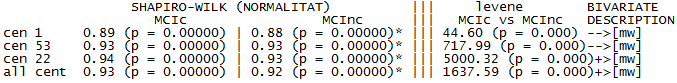
\includegraphics[width=1\textwidth]{fig_shapiro_levene_FCon.png}
			\caption{Assessment of the assumptions of all bivariate comparisons made in table \ref{fig:FCon_resultats}.}
			\label{fig:fig_shapiro_levene_FCon}
		\end{figure}
		\FloatBarrier
		\clearpage	
		
		
		
\section{Figures}

	\subsection{Unsuccessful models for functional connectivity without dimensionality reduction: ROC and Confusion matrices}\label{sec:fig_NaiveBayes_fMRI_nodimreduc_CONFUSIONiROCCURVE}

	
	\FloatBarrier
	%NAIVE BAYES ROC CURVE I CONFUSION MATRIX
	\begin{figure}[h]
		\centering
		\begin{minipage}{.5\textwidth}
			\centering
			\includegraphics[width=1\linewidth]{fig_GNB_fmri_nodimreduc_CONFUSION.png}
			\captionof{figure}{Naive Bayes confusion matrix.}
			%\label{fig:test1}
		\end{minipage}%
		\begin{minipage}{.5\textwidth}
			\centering
			\includegraphics[width=1\linewidth]{fig_GNB_fmri_nodimreduc_ROC.png}
			\captionof{figure}{Naive Bayes ROC curve.}
			%\label{fig:test2}
		\end{minipage}
	\end{figure}


	\FloatBarrier


	\begin{figure}[h]
		\centering
		\begin{minipage}{.5\textwidth}
			\centering
			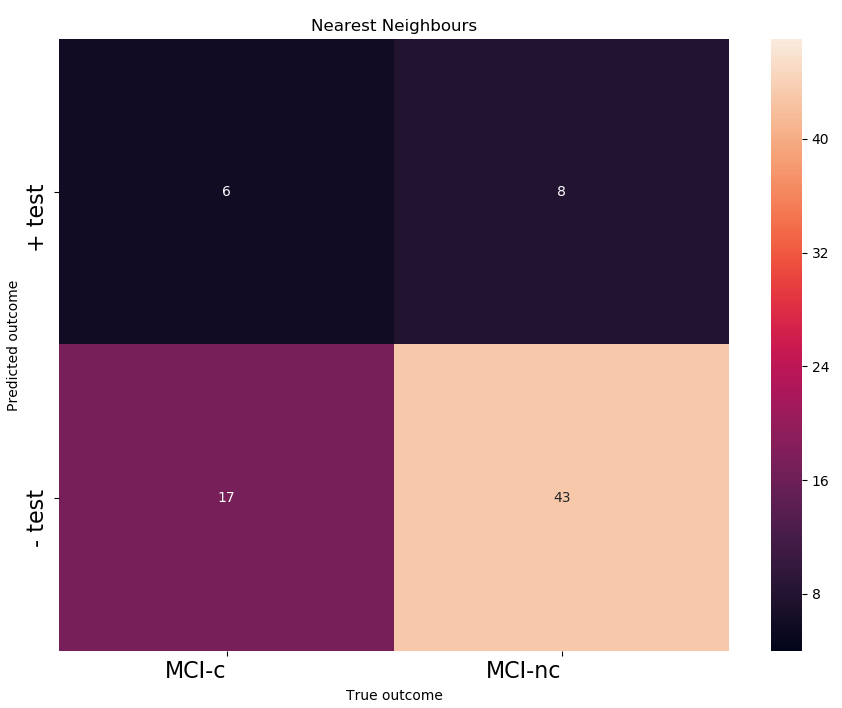
\includegraphics[width=1\linewidth]{fig_NN_fMRI_nodimreduc_CONFUSION.png}
			\captionof{figure}{Nearest Neighbours confusion matrix.}
			%\label{fig:test1}
		\end{minipage}%
		\begin{minipage}{.5\textwidth}
			\centering
			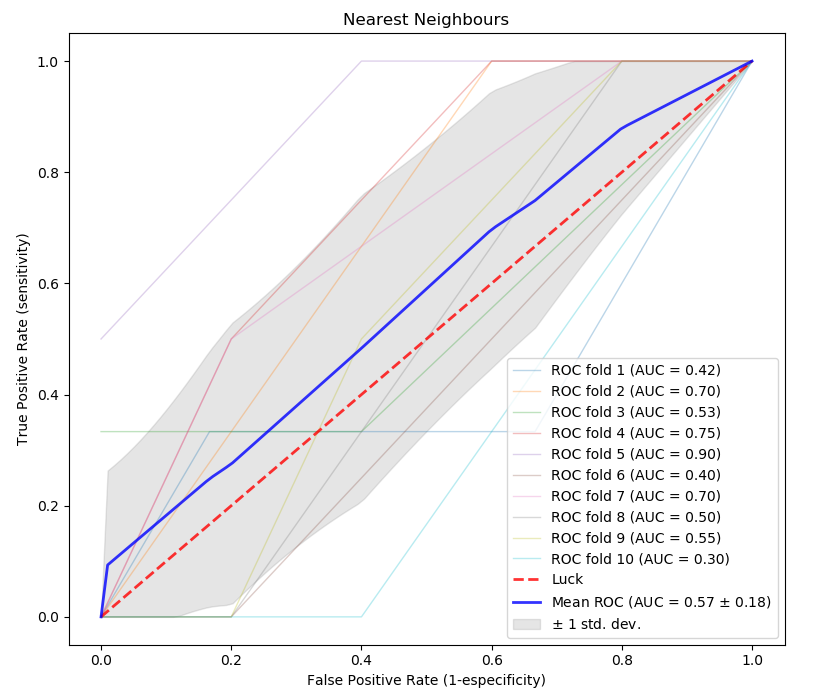
\includegraphics[width=1\linewidth]{fig_NN_fMRI_nodimreduc_ROC.png}
			\captionof{figure}{Nearest Neigbours ROC curve.}
			%\label{fig:test2}
		\end{minipage}
	\end{figure}





	\FloatBarrier
	
	\clearpage
	
	

	
	\subsection{Mean displacements for a randomly selected subject} \label{meandisplacements_registre}
		\FloatBarrier
		\begin{figure}[h]
			\centering
			\begin{subfigure}[a]{0.80\textwidth}
				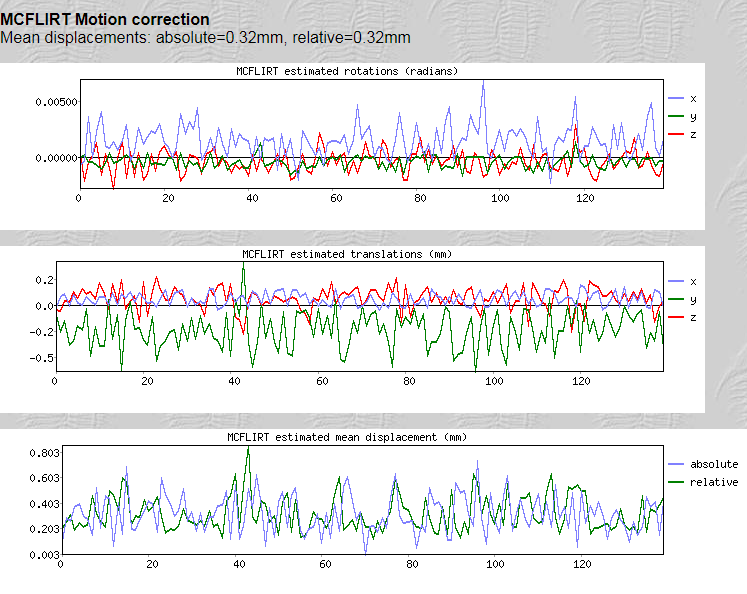
\includegraphics[width=1\textwidth]{fig_mean_displacements_annex.png}
				\caption{Preamble to motion-correction: Absolute mean displacement shows very good metrics.}
				\label{fig_mean_displacements_annex} 
			\end{subfigure}
			\begin{subfigure}[b]{0.80\textwidth}
				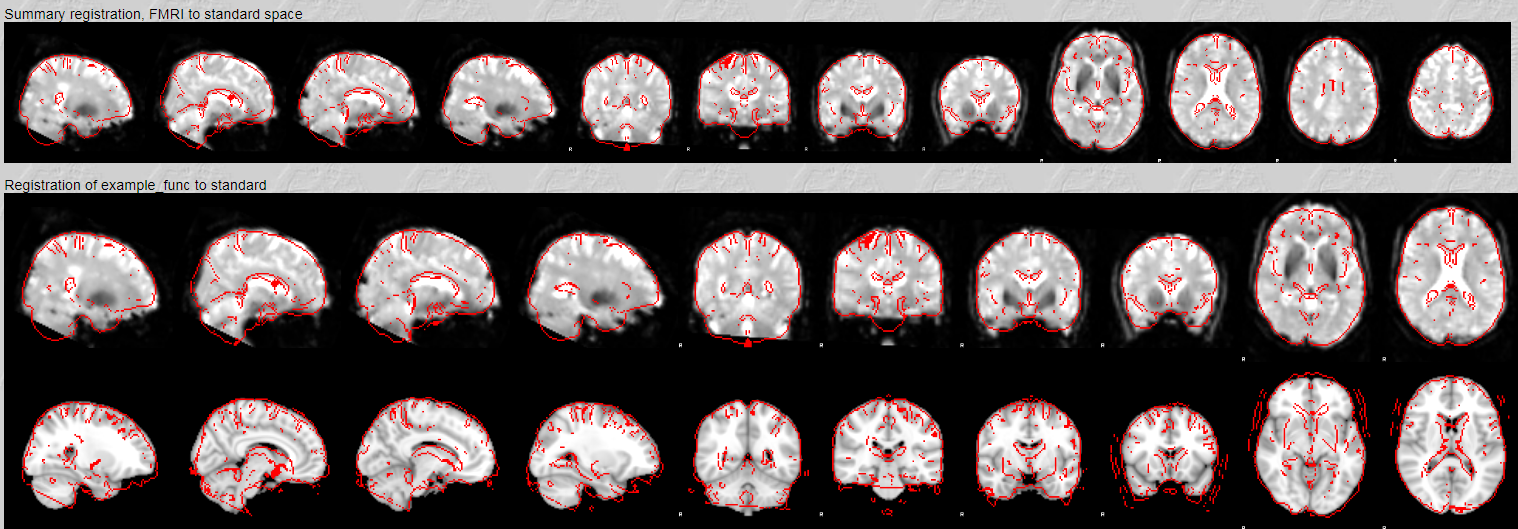
\includegraphics[width=1\textwidth]{fig_registre_cervellets.png}
				\caption{Registration information. GREY: Standard space. RED: the subject hereby considered. Both subjects are coincident.}
				\label{fig_registre_cervellets} 
			\end{subfigure}
			\caption{A randomly chosen subject from the 93 subjects whose fMRI scans were preprocessed using FSL.}
		\end{figure}
		\FloatBarrier
		\clearpage




	
		

\subsection{Functional connectivity matrices}\label{annex_functional_connectivities}

Here you can see the mean functional connectivity matrices across subject category (one for AD patients and the other for healthy controls), in the patients of the IDIBAPS clinic dataset (same dataset as \cite{Demirtas2017343}).


\begin{figure}[h]
	\centering
	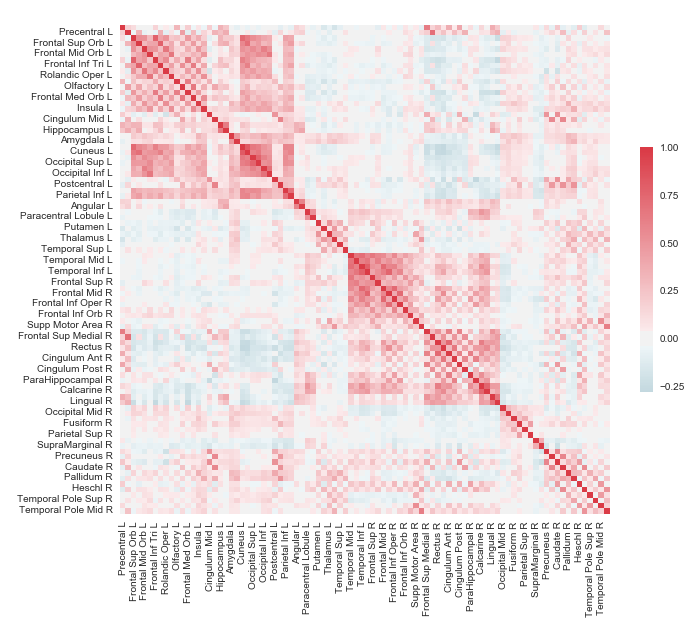
\includegraphics[width=\textwidth]{mitjana_ROIxROI_ALZHEIMER_ELIMINATS15PROBLEMATICS.png}
	\caption{Average correlation values for MNI AAL ROIs of Alzheimer disease patients}
\end{figure}


\begin{figure}[h]
	\centering
	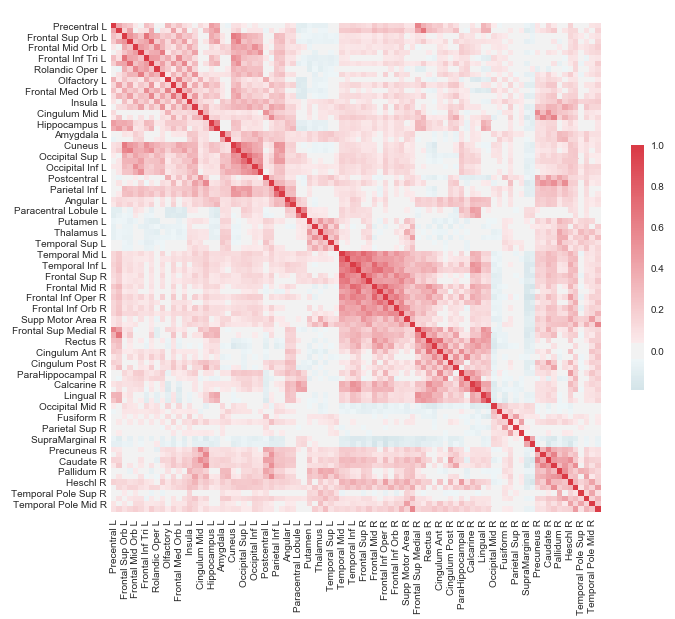
\includegraphics[width=\textwidth]{mitjana_ROIxROI_controls_ELIMINATS15PROBLEMATICS.png}
	\caption{Average correlation values for MNI AAL ROIs of healthy control patients}
\end{figure}


%REPORTING

\clearpage






	\section{Depicting the method of unique scan selection in subjects with more than one rsfMRI the same day} \label{escollir_escaners_repetits_dun_mateix_dia}

As we said, seven subjects had several scans in the same day: from these scans only one was to be chosen in order to test our hypothesis. We chose the best one according to the following criteria applied to figure \ref{fig:escans_exclosos}: 

BOLD:  Chosen scan $|$ CROSSED OUT: Excluded scan $|$ NO EMPHASIS: Scan eligible but not chosen because was not deemed to be the the most optimal.



\FloatBarrier
\begin{figure}[h]
	\centering
	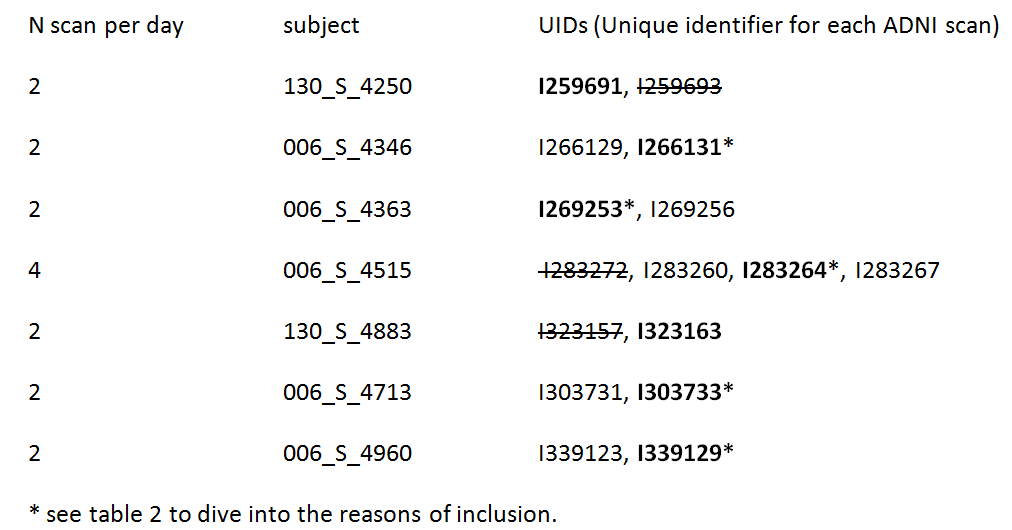
\includegraphics[width=\textwidth]{fig_escans_exclosos.png}
	\caption{Number of repeated rsfMRI scans in the same day, by subject and UID.}
	\label{fig:escans_exclosos}
\end{figure}
\FloatBarrier


The reasons why we directly excluded the scans that appear crossed out in figure \ref{fig:escans_exclosos} are:

a)	The scan was not completed (i.e. the scan had less than the number of time series –in this case 140- all the other subjects had): These is the problem found with I323157 and I283272 from subjects 130\_S\_4883 and 006\_S\_4515 respectively.

b)	FSL did not process the scan properly and did not even obtain an output file. The error shown on screen was ``WARNING:: Inconsistent orientations for individual images when attempting to merge'' and ``Error in size-match along non-concatenated dimension for input file:''  (besides in this case the scan did not even have information of fMRI adquisition parameters as an .xml file, whereas scans in the ADNI have a corresponding .xml file with those parameters). This  scan is I259693, corresponding to subject 130\_S\_4250. 

Sometimes exclusion was not straightforward, since several scans, apparently, were valid candidates to represent the functional connectivity of a given subject. Thus, for each of those given subjects,  we simply chose the representing scan based on a criteria of minimizing the absolute and relative mean displacements as showed in the “report.html” file Melodic obtains for each subject that the software preprocesses. This is the case for  the subjects  006\_S\_4346,  006\_S\_4363,  006\_S\_4713,  006\_S\_4960. For this subjects we provide the mean displacements as follows in figure \ref{fig:escans_displacements}:


\FloatBarrier
\begin{figure}[h]
	\centering
	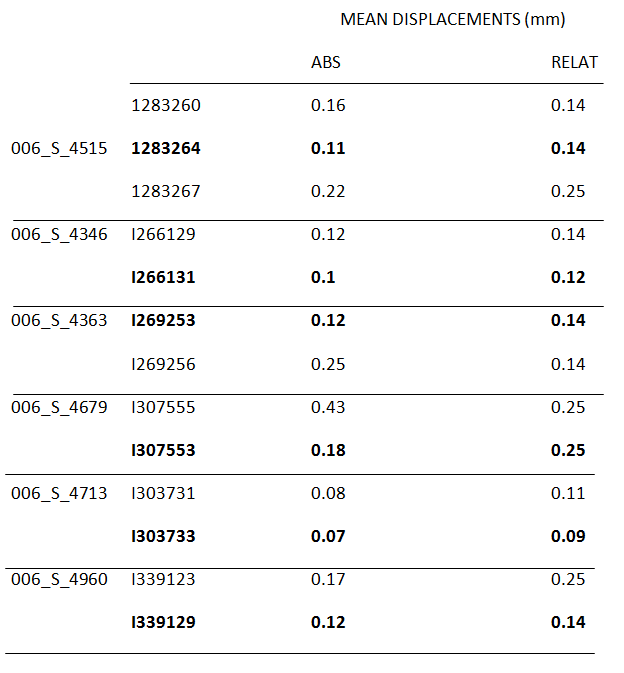
\includegraphics[width=0.8\textwidth]{fig_escans_displacements.png}
	\caption{NOTE: Mean absolute and relative displacements for scans of subjects taken in the same day. One scan was selected per each subject for having the lowest mean displacements. $|$ \textit{NOTE: Although scan I259691 did not have fMRI adquisition parameters as an .xml, it was not excluded. We assumed same parameters as other scans.}}
	\label{fig:escans_displacements}
\end{figure}
\FloatBarrier
\clearpage















\section{Reporting: EQUATOR guidelines} \label {equator_guidelines}

\subsection{Creating a tailored guideline for our study}
In this final thesis I chose the {TRIPOD checklist, in its prediction model development and validations version}, to report my results (\href{https://bit.ly/2HU58V5}{click here} to see them \footnote{or copy the following footnote adress https://bit.ly/2HU58V5}). However, since this study has some particularities that regular prognostic studies do not have, some features were uncovered and not asked to be reported. 

To overcome this limitation, I decided to add three extra guidelines. First, the STARD guidelines, that are used in diagnostic studies; Second, the MLBS guidelines\footnote{These guidelines do not have an oficial abreviation. We have created one that stands for Machine Learning in the Biomedical Sciences.}, to report correctly the created machine learning models in our study, since their complexity makes it harder to convey good reporting; and finally, the RECORD guidelines, in order to properly specify the process of obtaining the information from a database fed with routinely collected data from observational studies (the ADNI belongs to that category, since it is a cohort study with regular follow-ups).

The EQUATOR links for the guidelines used can be found and explained in the following table:

\begin{center}
	\begin{table}[h] 
		\begin{tabular}{m{3cm} m{9.8cm}}
			\hline
			\textbf{Guideline\newline abbreviation} & \textbf{repoting\newline aim}\\
			\hline
			\href{http://www.equator-network.org/reporting-guidelines/tripod-statement/}{TRIPOD} & Studies developing, validating, or updating a prediction model, whether for diagnostic or prognostic purposes.\\
			\hline
			\href{http://www.equator-network.org/reporting-guidelines/stard/}{STARD} & Diagnostic accuracy studies\\
			\hline
			\href{http://www.equator-network.org}{RECORD} & Reporting items specific to observational studies using routinely collected health data.\\
			\hline
			\href{http://www.equator-network.org/reporting-guidelines/guidelines-for-developing-and-reporting-machine-learning-predictive-models-in-biomedical-research-a-multidisciplinary-view/}{MLBS}$^{***}$ & Machine learning predictive models in biomedical research\\
			
			\hline	
		\end{tabular}{}
		\caption{EQUATOR guidelines that have been used for reporting this pronostic study. $^{***}$ \textit{These guidelines do not have an oficial abreviation. We have created one, that stands for Machine Learning in the Biomedical Sciences}}
	\end{table}
\end{center}

%\section{Codes and syntaxis files} 

%In this section python code can be followed to see how we approached the data analysis. We have not been exhaustive in all the functions shown, because the list of codes has several files. This is just for display the most relevant parts of the code.


%\subsection{finding NaNs within a 3D tensor}\label{codis}
%\lstinputlisting[language=python]{inputlatexprovapython.py}


%\subsection{main function for analysis}
%\lstinputlisting[language=python]{./copiescodi/funcionsauxiliars.py}



\section{Director/tutor final thesis certificate} \label{director}

\FloatBarrier
\begin{figure}[h]
	\centering
	
\includegraphics[width=1\textwidth]{fig_certificat_tutoridirector.png}
	\label{fig:tutordirector}
\end{figure}
\FloatBarrier
\clearpage





